%
\section{Studying MSE values through analysis of Bias-variance}
%
% Set background color and other options for lstlisting

\hfill\break
The main code is obtained from: \url{https://compphysics.github.io/MachineLearning/doc/LectureNotes/_build/html/chapter3.html#the-bias-variance-tradeoff.}
\hfill\break
Modified code uses $y=sin(x)+log(x^2)$ as the one-dimensional function.


    \begin{lstlisting}[language=Python]
    import matplotlib.pyplot as plt
    import numpy as np
    from sklearn.linear_model import LinearRegression, Ridge, Lasso
    from sklearn.preprocessing import PolynomialFeatures
    from sklearn.model_selection import train_test_split
    from sklearn.pipeline import make_pipeline
    from sklearn.utils import resample

    np.random.seed(2018)

    n = 40
    n_boostraps = 100
    maxdegree = 14


    # Make data set.
    x = np.linspace(-3, 3, n).reshape(-1, 1)
    y = np.sin(x) + np.random.normal(0, 0.1, x.shape)
    error = np.zeros(maxdegree)
    bias = np.zeros(maxdegree)
    variance = np.zeros(maxdegree)
    polydegree = np.zeros(maxdegree)
    x_train, x_test, y_train, y_test = train_test_split(x, y, test_size=0.2)

    for degree in range(maxdegree):
        model = make_pipeline(
            PolynomialFeatures(degree=degree), LinearRegression(fit_intercept=False)
        )
        y_pred = np.empty((y_test.shape[0], n_boostraps))
        for i in range(n_boostraps):
            x_, y_ = resample(x_train, y_train)
            y_pred[:, i] = model.fit(x_, y_).predict(x_test).ravel()

        polydegree[degree] = degree
        error[degree] = np.mean(np.mean((y_test - y_pred) ** 2, axis=1, keepdims=True))
        bias[degree] = np.mean((y_test - np.mean(y_pred, axis=1, keepdims=True)) ** 2)
        variance[degree] = np.mean(np.var(y_pred, axis=1, keepdims=True))
        print("Polynomial degree:", degree)
        print("Error:", error[degree])
        print("Bias^2:", bias[degree])
        print("Var:", variance[degree])
        print(
            "{} >= {} + {} = {}".format(
                error[degree],
                bias[degree],
                variance[degree],
                bias[degree] + variance[degree],
            )
        )

    plt.plot(polydegree, error, label="Error")
    plt.plot(polydegree, bias, label="bias")
    plt.plot(polydegree, variance, label="Variance")
    plt.legend()
    plt.show()
    \end{lstlisting}
Results from the bias and variance trade-off as function of the model complexity can be seen in the table ~\ref{tab:ModelComplexMSE} below.
Here we set the number of data points to 40 and bootstrap to 100 iterations.
Blue rows highlights where the model complexity yields the lowest error:

\begin{table}
    \centering
    \begin{tabular}{c|c|c|c}
        \textbf{Order} & \textbf{Error} & \textbf{Bias\textsuperscript{2}} & \textbf{Variance}\\
        \text{0} & 3.222694  & 3.104592   & 0.118102\\
        \text{1} & 2.637989  & 2.492254   & 0.145734 \\
        \text{2} & 1.234957 & 1.095855    & 0.139102\\
        \text{3} & 1.142538 & 0.978143   & 0.164395\\
        \text{4} & 0.604439 & 0.475311  & 0.129127\\
        \text{5} & \cellcolor{blue!25}0.578585 & \cellcolor{blue!25}0.4131747   & \cellcolor{blue!25}0.165410\\
        \text{6} & \cellcolor{blue!25}0.370845 & \cellcolor{blue!25}0.214435   &  \cellcolor{blue!25}0.156410\\
        \text{7} & \cellcolor{blue!25}0.435129 & \cellcolor{blue!25}0.229928  & \cellcolor{blue!25}0.205200\\
        \text{8} & 0.739773 & 0.360638   & 0.379134\\
        \text{9} & 1.179098 & 0.368951   & 0.810147 \\
        \text{10} & 0.917037& 0.390615   & 0.526421 \\
        \text{11} & 7.420075 & 0.278572  & 7.141503  \\
        \text{12} & 9.530186 & 0.267499  & 9.262687  \\
        \text{13} & 16.252874 & 0.147212 & 16.105661 \\
    \end{tabular}
    \caption{Bias and variance trade-off as function of polynomial complexity.}
    \label{tab:ModelComplexMSE}
\end{table}

\begin{figure}
    \centering
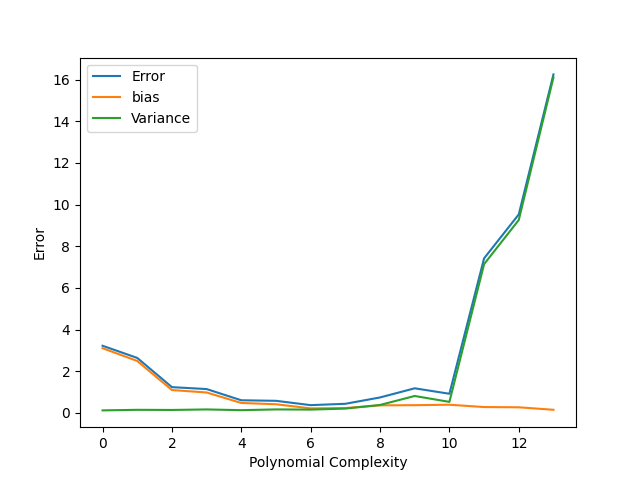
\includegraphics[width=1.0\linewidth]{FYS-STK4155/figures/Figure_1.png}
    \caption{Plot Analysis of  plot of error, bias, and variance as function of increasing complexity}
    \label{fig:1}
\end{figure}

\newpage
\section{Bias-Variance Trade-Off}
%
\begin{itemize}
    \item \textbf{Low Complexity($<5$):} High bias and low error, the model underfits our test data and is not able to capture the complexity of our target function. This gives us a somewhat higher error.
    \item \textbf{Optimal Complexity($5-7$):} Our error is relatively low meaning that our model does a decent job in describing underlying patterns in the target function. This is provided by the bias-term. The variance on the other hand, is low enough so our model does not overfit. For the polynomial degree between 4-7 we can see that the trade-off between bias and variance is minimizes the error.
    \item \textbf{High Complexity($>7$):} The low bias describes now that our model is exceptional at fitting to our target function, but our model is now too specific - it is restricted to perform well with the data set we provided, but will struggle with new data sets. The high variance shows that our model has been overfitted and the higher error describes that our model is no longer suitable for generalization.
\end{itemize}
%
From the table we can see the error of the model is at its lowest when the degree of the polynomial is 6. This also holds true for visual inspection of the graph in figure ~\ref{fig:1}.

\section{Effect of Number of Data Points}

\hfill\break
From quick plots we observed that for low function complexity, the error, bias and variance stayed low (closer to $0$, seemingly). A major difference is the magnitude of error. On the y-axis we observed the error for (data points = 10) to take values between 0-700. When setting number of data points to 70, the error decreased and was within the range 0-3.5, but the error, bias and variance stayed at an all time low of zero until a polynomial degree of 10.

\section{Bootstrap Resampling}
As for bootstrap resampling we worked with the following number of bootstraps while holding number of samples fixed: (10,200).
For number of bootstraps= 10 the error varied where the bias was approximate close to the error to begin with. The graph of bias and errors stayed the same until degree 11 where error and variance were dominant and closer to each other and suddenly made a jump(see~\ref{fig:2}).
As for number bootstrap= 200, we had another behaviour. As depicted in figure~\ref{fig:3}.

\begin{figure}
    \centering
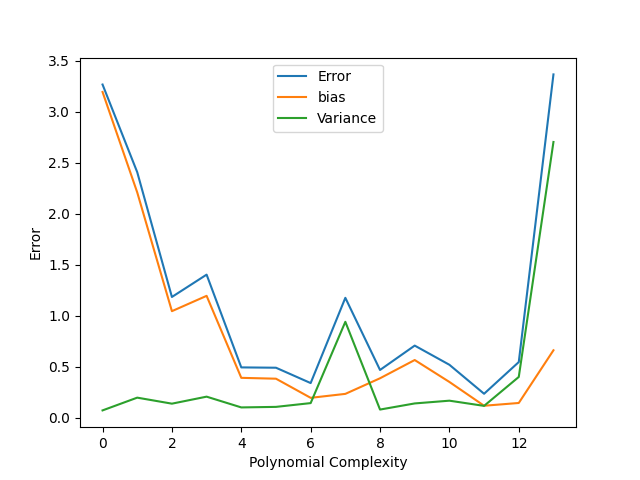
\includegraphics[width=1.0\linewidth]{FYS-STK4155/figures/bootstrap 1.png}
    \caption{Plot Analysis of  plot of error, bias, and variance as function of increasing complexity}
    \label{fig:2}
\end{figure}

\begin{figure}
    \centering
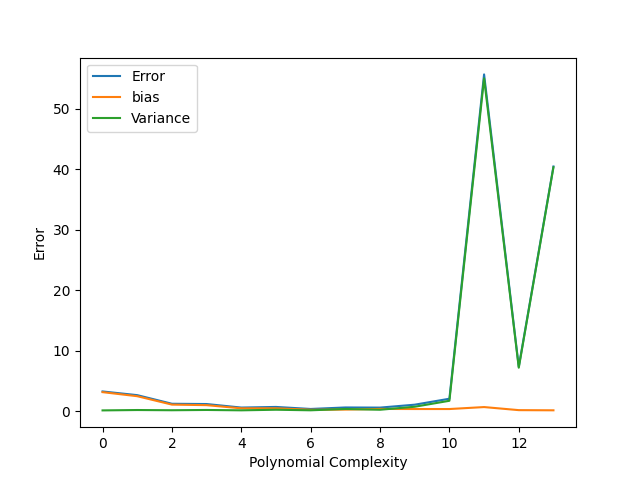
\includegraphics[width=1.0\linewidth]{FYS-STK4155/figures/bootrstrap2.png}
    \caption{Plot Analysis of  plot of error, bias, and variance as function of increasing complexity}
    \label{fig:3}
\end{figure}

